%%%%%%%%%%%%%%%%%%%%%%%%%%%%%%%%%%%%%%%%%%%%%%%%%%%%%%%%%%%%%%%%%%
%  = PREAMBLE =
% The preamble of a LaTeX document is the set of commands that 
%    precede the \begin{document} line.  It sets up the style of 
%    the document.
%%%%%%%%%%%%%%%%%%%%%%%%%%%%%%%%%%%%%%%%%%%%%%%%%%%%%%%%%%%%%%%%%%

\documentclass[aps,twocolumn, secnumarabic,balancelastpage,amsmath,amssymb,nofootinbib,floatfix]{revtex4-1}

\usepackage{graphicx}      % tools for importing graphics
\usepackage{parskip}
\usepackage[colorlinks=true]{hyperref}  % this package should be added after 
                                        % all others.
                                        % usage: \url{http://web.mit.edu/8.13}

\setlength{\parskip}{5pt}
%%%%%%%%%%%%%%%%%%%%%%%%%%%%%%%%%%%%%%%%%%%%%%%%%%%%%%%%%%%%%%%%%%%
% And now, begin the document...
%%%%%%%%%%%%%%%%%%%%%%%%%%%%%%%%%%%%%%%%%%%%%%%%%%%%%%%%%%%%%%%%%%%

\begin{document}

\title{Michelson Experiment Summary}
\author{Yongao Hu}
\email{yongao@mit.edu}
\date{\today}
\affiliation{MIT Department of Physics}


\begin{abstract}
This report presents the results of the Michelson interferometer experiment conducted in MIT Junior Lab during Spring 2025. The objective of the experiment was to measure the wavelength of a light source. The experiment was successful in demonstrating the principles of interference and the wave nature of light. The wavelength of the orange laser was found to be $601\pm37(\text{sys})\pm10(\text{stat})\text{ nm}$ and the visibility of the interference pattern was found to be $0.179\pm0.001(\text{stat})$. 
\end{abstract}

\maketitle

\section{Introduction}
Light, having the properties of a wave, exhibits interference patterns when two light waves overlap. Interference patterns can be used to measure small distances. The interferometer is based on the principle of interference of light waves. In particular, the Michelson interferometer, designed by Albert Michelson, is used to measure the wavelength of light \cite{MichelsonMorley1887}. Historically, the Michelson interferometer was used to disprove the existence of the ''luminiferous aether'' \cite{MichelsonMorley1887}, paving the way for the theory of relativity \cite{MITOpticalInterferometry2023}. The Michelson interferometer is also widely used in physics to measure small distances and to detect small changes in the refractive index of the medium \cite{MITOpticalInterferometry2023}. Specifically, a variant of the Michelson interferometer was used in the LIGO experiment to detect gravitational waves \cite{LIGO2016}.

The Michelson interferometer comprises a beam splitter, two mirrors, and a detector \cite{MichelsonMorley1887,MITOpticalInterferometry2023}. The beam splitter splits the light beam into two beams. The two beams travel different paths and are reflected back by the mirrors. The two beams are then recombined at the beam splitter. The interference pattern is then detected by the detector. 

\section{Theory: Interference of Light Waves}
\subsection{Interference of Light Waves}
The Michelson interferometer is based on the principle of interference of waves. The interference pattern is determined by the phase difference between the two waves. For two sinusoidal waves of the same wavelength $\lambda$, the phase difference is given by
\begin{equation}
\Delta \phi = 2\pi \frac{\Delta x}{\lambda}
\end{equation}
where $\Delta x$ is the path difference between the two waves. The interference pattern is given by
\begin{equation}
    I = I_0 \cos^2(\Delta \phi)
\end{equation}
where $I_0$ is the intensity of the light source.

The interference pattern has \textit{primary maxima} when $\Delta \phi = 2\pi n$ and \textit{primary minima} when $\Delta \phi = (2n+1)\pi$, where $n$ is an integer. 

\subsection{Visibility of the Interference Pattern}

Additionally, ensuring the interference pattern is well resolved is crucial. The \textit{visibility} of the interference pattern measures how well the interference pattern is resolved. The visibility is given by:
\begin{equation}
    V = \frac{I_{\text{max}} - I_{\text{min}}}{I_{\text{max}} + I_{\text{min}}}
\end{equation}
where $I \propto V_{\text{diode}}$. 

In theory, if lasers are aligned perfectly, the visibility of the interference pattern should be $1$. If the visibility is low, the primary maxima and minima are close in intensity, making them difficult to distinguish. 

\subsection{Piezoelectric Transducer to Change Path Difference}
In order to change the path difference $\Delta x$ by a small amount, we use a \textit{piezoelectric transducer} to move one of the mirrors \cite{MITOpticalInterferometry2023}. A piezoelectric transducer is an electronic device that deforms when a voltage is applied \cite{PiezoFilm2006}. The piezoelectric device we are using in particular changes its length when a voltage is applied, moving the attached mirror by length $\Delta L$.  The change in length is proportional to the voltage applied \cite{MITOpticalInterferometry2023}. 

When we apply different voltages to the piezoelectric device, we change the path difference $\Delta x$ between the two waves, changing the interference pattern as a result. By recording the voltage corresponding to the maxima and minima of the interference pattern, we can determine the average $\Delta V$ between consecutive extrema. 

We can then calculate the path difference between the two waves. Note that since we are using a beam splitter and mirrors to reflect the light, the change in path difference is twice the change in length of the piezoelectric device. Since the change in path difference between consecutive maxima and minima is $\lambda/2$, the change in length of the piezoelectric device is $\lambda/4$.
The wavelength of the light source is then given by:
\begin{equation}
    \lambda = 4 \Delta V \times \frac{\Delta L}{V} 
    \label{eq:wavelength}
\end{equation}


\section{Experimental Design}
The experiment was conducted using the Michelson interferometer setup at MIT Junior Lab in Feburary 2025 \cite{MITOpticalInterferometry2023}. The light source is a laser. The beam splitter was a 50/50 beam splitter. One mirror is stationary, while the other mirror is mounted on a piezoelectric transducer. The piezoelectric device we use is calibrated to have the length-voltage ratio of:
\begin{equation}
     \frac{\Delta L}{V} = (47.1\pm2.9) \text{ nm/V}
     \label{eq:calibration}
\end{equation}
The detector is a photodiode. The voltage output of photodiode is proportional to the intensity of the light on the detector. We used a signal generator to apply a triangular voltage of amplitude of $10 \text{ V}$ and frequency of $10 \text{ Hz}$ to the piezoelectric transducer. The schematic of the setup is shown in Fig. \ref{fig:set_up}.

The applied voltage altered the path difference $\Delta x$. We recorded the signal generator voltage and the photodiode voltage. 
\begin{figure}[h]
    \centering
    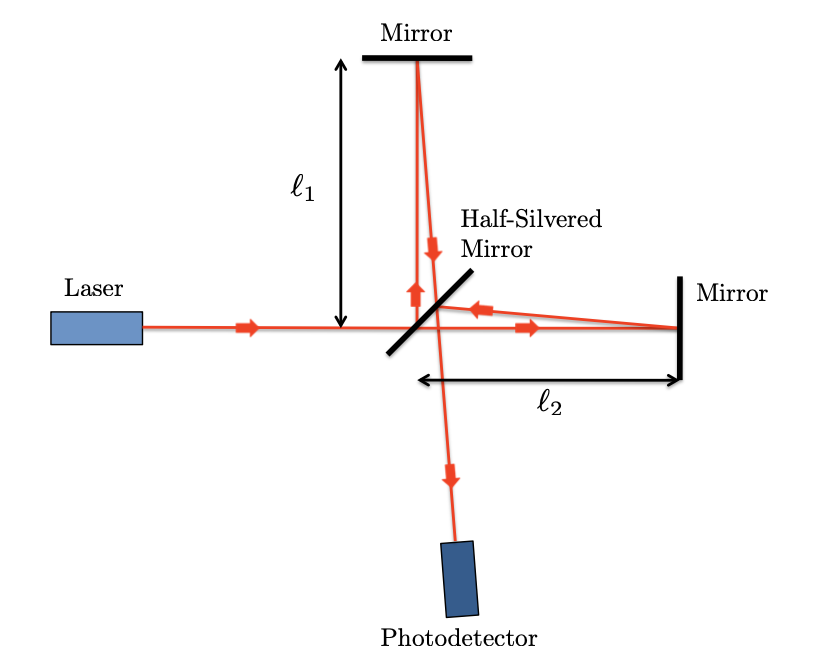
\includegraphics[width=0.45\textwidth]{fig/michelson_setup.png}
    \caption{The set up of the Michelson interferometer. The figure is reproduced from \cite{MITOpticalInterferometry2023}. The light source is a laser. The beam splitter is a 50/50 beam splitter. The mirror to the right of the beam splitter is mounted on a piezoelectric transducer. The other mirror is stationary. The detector is a photodiode. The signal generator applies a triangular voltage to the piezoelectric transducer to change the path length.}
    \label{fig:set_up}
\end{figure}

\section{Data Analysis}
We obtained the voltages of signal generator and photodiode against time from the output of the oscilloscope. We tabulated the voltage of the signal generator and the voltage of the photodiode. We then used the \texttt{findpeak} function of \texttt{SciPy} to find the primary maxima and minima of the photodiode voltage. In order to filter out the secondary maxima and minima that occurs when the triangular input voltage changes direction, we chose the prominence of the peaks to be $0.4$. 

We acknowledge that the choice of peak prominence is an arbitrary choice; some primary maxima and minima might have been missed, particularly in regions of lower visibility. We will discuss the impact of this choice in the results section.

To cluster different bands of the signal generator voltage and identify neighboring primary maxima and minima, we used the \texttt{KMeans} clustering algorithm from \texttt{SciKit-Learn}. We then calculated the average voltage difference between the consecutive primary maxima and minima. The wavelength of the light source is then given by Eq. \eqref{eq:wavelength}. 


\section{Results}
\subsection{Visibility of the Interference Pattern}

Figure \ref{fig:intensity} shows the photodiode intensity at different voltages. The average maximum voltage is found to be $(1.592\pm0.002(\text{stat})) \text{ V}$ and the average minimum voltage is found to be $(1.110\pm0.002(\text{stat})) \text{ V}$. The visibility of the interference pattern is found to be $0.179\pm0.001(\text{stat})$.
\begin{figure}[h]
    \centering
    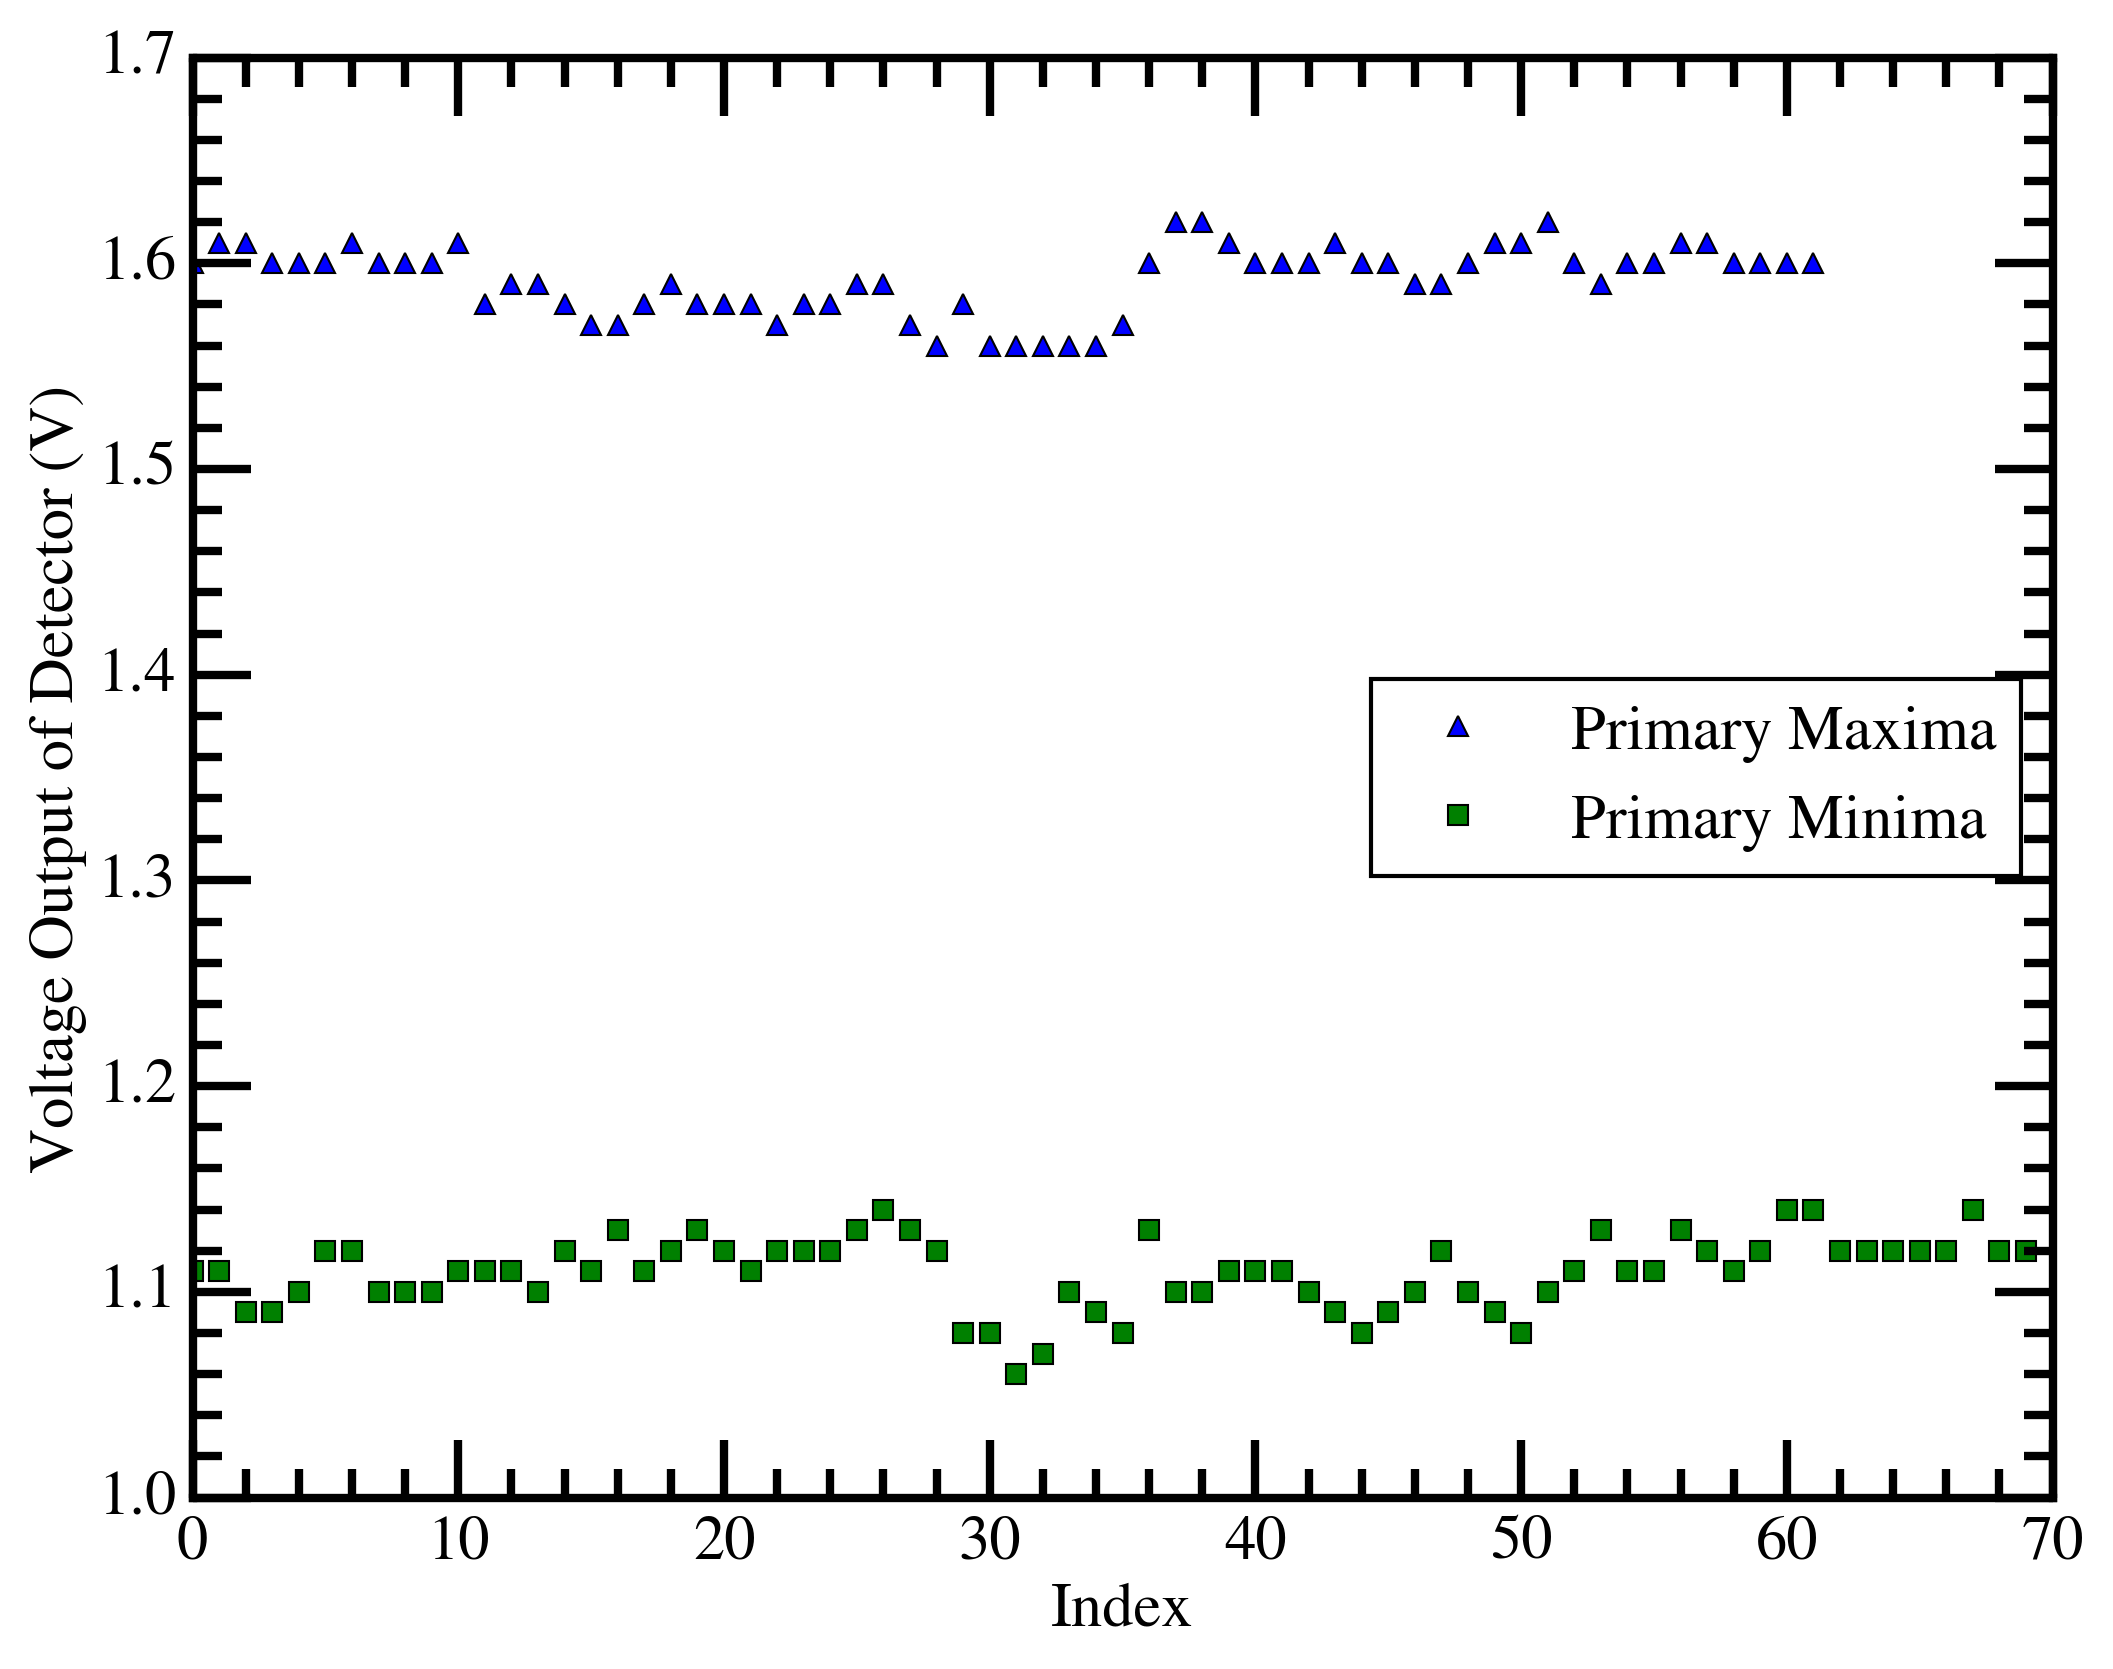
\includegraphics[width=0.45\textwidth]{fig/Intensity.png}
    \caption{The voltage output of the photodiodes that correspond to primary maxima and minima. The blue triangles represent the primary maxima and the green squares represent the primary minima. We can see that the primary maxima and minima correspond to approximately constant photodiode voltage (constant intensity). The error bars are negligible due to the resolution of the oscilloscope.}
    \label{fig:intensity}
\end{figure}

The visibility of $0.179$, smaller than $1$, indicates that the alignment of the mirrors is not perfect. The misalignment of the setup could be that the mirrors not being perfectly aligned with the beam splitter and the laser source.

Figure \ref{fig:intensity} shows that some primary minima and maxima were missed, particularly in the maxima beyond index 60. This is likely due to the lower visibility of the interference pattern at those points. As a result, we have fewer primary maxima and minima, increasing the statistical uncertainty of the visibility. However, we have not included the secondary maxima and minima in the analysis, which would have increased the systematic uncertainty of the visibility. 


\subsubsection{Uncertainty of Visibility}
The uncertainty of the visiblity comes from the statistical uncertainty of the maximum and minimum voltage, calculated in the standard way of $\sigma/\sqrt{N}$. We then used the usual formula of error propagation to find the uncertainty of the visibility. The uncertainty of the visibility is found to be $0.001$. 

The systematic uncertainty in visibility primarily arises from photodiode calibration and oscilloscope resolution, though these contributions are negligible compared to statistical uncertainty. We did not explicitly include the systematic uncertainty of the visibility into the final result.

\subsection{Wavelength of the Light Source}
The voltages of the signal generator at primary maxima and minima are shown in Fig. \ref{fig:data}. 
\begin{figure}[h]
    \centering
    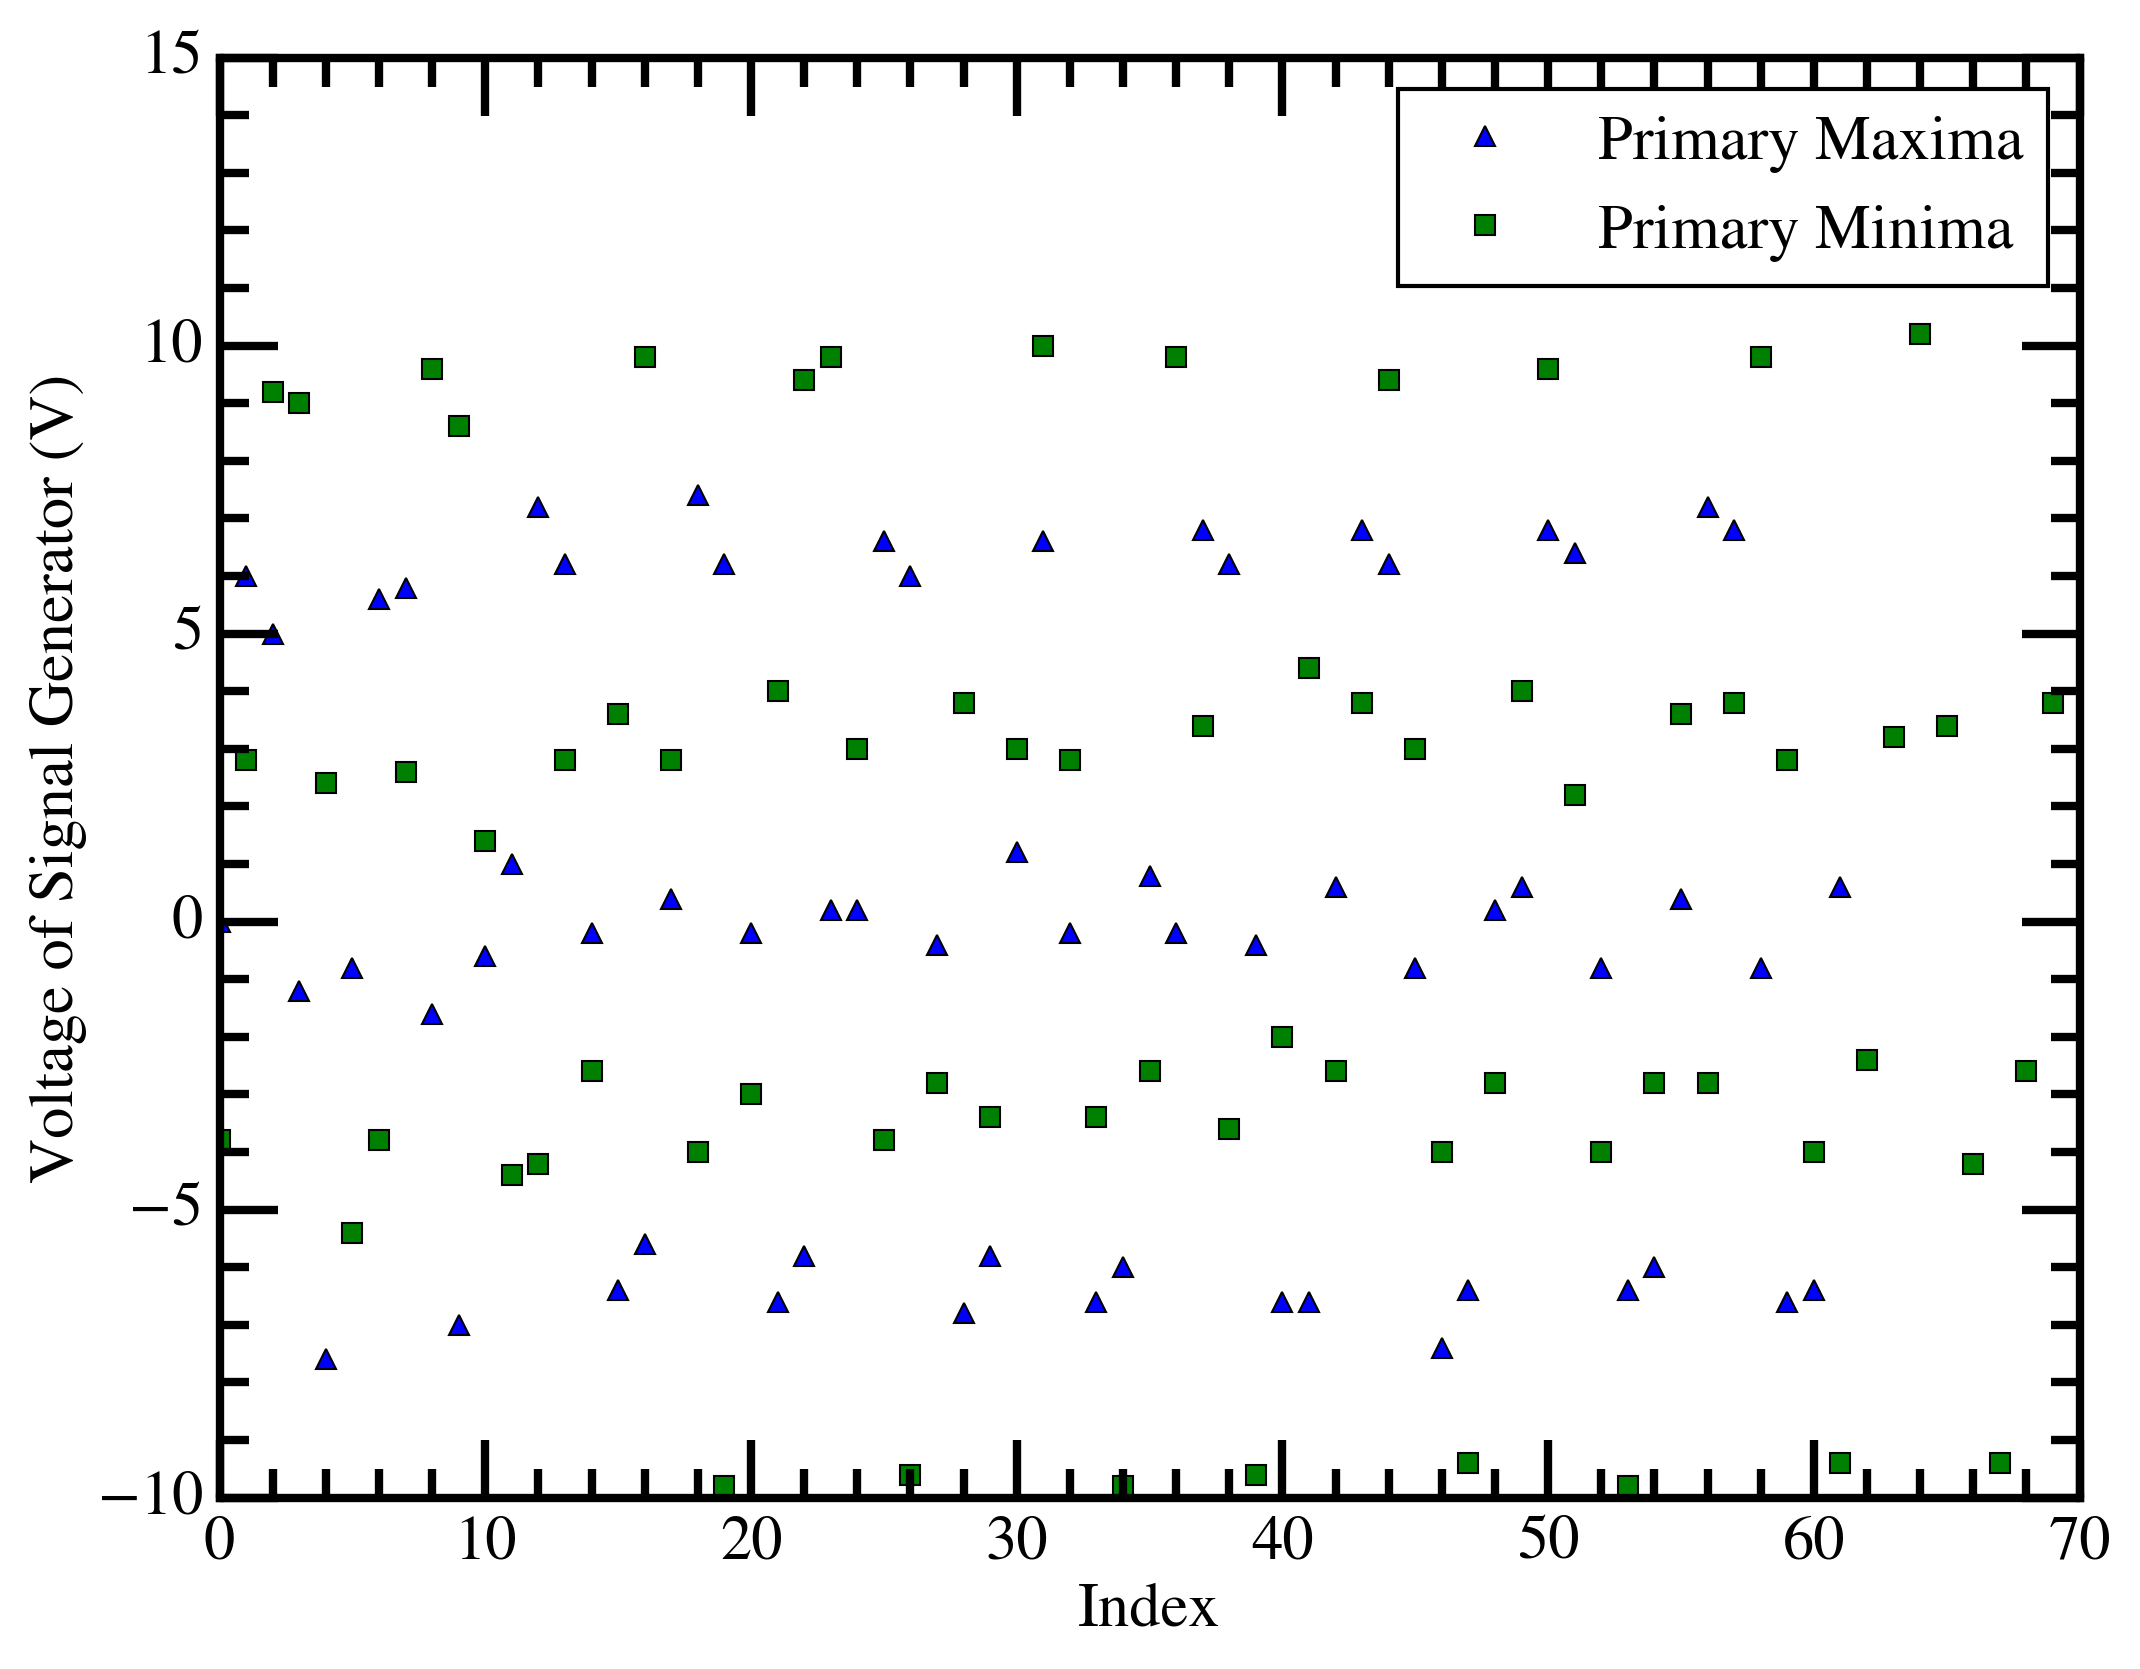
\includegraphics[width=0.45\textwidth]{fig/Primary_Maxima_Minima.png}
    \caption{The voltages corresponding to primary maxima and minima. The blue triangles represent the primary maxima and the green squares represent the primary minima. We can visually see that the primary maxima and minima are clustered into 3 and 4 bands, respectively. The error bars are negligible due to the resolution of the oscilloscope.}
    \label{fig:data}
\end{figure}

The clustering algorithm identified 3 clusters of primary maxima and 4 clusters of primary minima. The values of the signal generator voltage at primary maxima and minima are shown in Table \ref{tab:minima_maxima}. The average voltage between the primary maxima and minima are $(3.192 \pm 0.055 (\text{stat})) \text{ V}$. 

\begin{table}[h]
    \centering
    \begin{tabular}{|c|c|}
        \hline
        \textbf{Voltage at Minima (V)} & \textbf{Voltage at Maxima (V)} \\
        \hline
        $-9.60 \pm 0.06$ & $-6.48 \pm 0.12$ \\
        \hline
        $-3.40 \pm 0.16$ & $-0.08 \pm 0.14$ \\
        \hline
        $3.18 \pm 0.14$  & $6.41 \pm 0.13$  \\
        \hline
        $9.55 \pm 0.12$  &  \\
        \hline
    \end{tabular}
    \caption{The voltage of signal generator at primary maxima and minima after clustering. The errors come from the standard deviation of the data points in the cluster. We can then calculate the average voltage between consecutive primary maxima and minima to calculate the wavelength of the light source.}
    \label{tab:minima_maxima}
\end{table}

The wavelength of the light source is then found to be $601\pm37(\text{sys})\pm10(\text{stat})\text{ nm}$. The wavelength corresponds to the orange light, which is consistent with the color of the laser that we used.

\subsubsection{Uncertainty of Wavelength}
The systematic error of the experiment is mainly due to the calibration of the piezoelectric device. The calibration of the piezoelectric device is given by Eq. \eqref{eq:calibration}. The uncertainty of the calibration is $2.9 \text{ nm/V}$. The systematic uncertainty of the wavelength is then given by:
\begin{equation}
    \delta \lambda = \lambda \left(4 \Delta V \times  \frac{\delta \Delta L / V}{\Delta L/V}\right) \approx 37 \text{ nm}
\end{equation}

The statistical error of the experiment mainly comes from the variation of different primary maxima and minima. We used the usual statistical approach of $\sigma/\sqrt{N}$ to estimate the uncertainty of the average $\Delta V$. The uncertainty of the average $\Delta V$ is $0.055 \text{ V}$. The statistical uncertainty of the wavelength is then given by:
\begin{equation}
    \delta \lambda = \lambda \left(4 \frac{\delta \Delta V}{\Delta V} \times \frac{\Delta L}{V}\right) \approx 10 \text{ nm}
\end{equation}
 

\section{Conclusion}
The Michelson interferometer experiment was successful in measuring the wavelength of the light source. The wavelength of the orange laser was found to be $(601\pm37(\text{sys})\pm10(\text{stat}))\text{ nm}$. The visibility was found to be $0.179\pm0.001(\text{stat})$. The experiment successfully demonstrated the principles of interference and the wave nature of light. To improve the experiment, we could use some form of feedback to adjust the mirrors automatically for better alignment. Moreover, we could use a more precise piezoelectric device to change the path difference. 

\begin{acknowledgments} The author gratefully acknowledges J. Lewis and M. Bohdan for their invaluable help in conducting the experiment. The author also acknowledges their lab partner V. Tran for their assistance in data analysis. The author also thanks the 8.13 teaching team for their guidance in the lab. This work was supported by the MIT Department of Physics. 
\end{acknowledgments}

\bibliographystyle{abbrv}
\bibliography{report_michelson_ref}
\end{document}

